\chapter{Cloud-SAP}

\chapterintro{ This chapter introduces the reference architecture known as Cloud-SAP, highlights its core concepts and indicates possible implementation ideas.
}

\section{Motivation}
As one can see, latest advances in providing platform-as-a-service still do not yield a comprehensive solution that embraces a range of fine-grained actions relevant to a given situation in an environment, as it was summarised in previous chapter. All of the presented solutions solely engage horizontal scaling, while other IT processes and corresponding actions such as vertical scaling, cloud bursting or application platform restart remains neglected. What is more, none of the investigated systems is a self-managing one, taking passive approach in enforcing given QoS. To make matter worse, some platforms such as Carina or OneFlow are provider-specific, hence, requiring vast knowledge and time.

What system has all of the above-mentioned features is an autonomic one \cite{IBM06}, characterised by a self-management ability and driven by a four crucial attributes:
\begin{itemize}
 \item \emph{self-configuration} - dynamic adaptation to changing environment such as provisioning new application instances, application tuning, traffic delegation to an external provider
  \item \emph{self-healing} - discovering, diagnosing and reacting to environment disruption such as container outage
  \item \emph{self-optimising} - monitoring and tuning resources: migrating containers, offloading traffic, for example
  \item \emph{self-protecting} - detecting and protecting against threats such as Deny-of-Service by provisioning extra resources
\end{itemize}

Another indispensable function of any autonomic entity is its ability to detect an undesirable state and take appropriate actions. This is achieved by the presence of a \emph{control loop} which collects data about the environment, analyzes it and takes all needed steps. Not only can the introduced attributes be bound to an autonomic system, but they can also be thought of main and broad categories of a control loop \cite{IBM06}.

Beside this, key customer values such as IT process execution cost or time needed to complete it are enhanced through rapid process initiation and reduced time and skill requirements \cite{IBM06}. As specified in blueprint, applying autonomic system to manage application environment is possible because following conditions are met:
\begin{itemize}
  \item tasks involved in associated IT process needs to be automated
  \item it is possible to initiate processes based on observable and detectable situations
  \item autonomic manager posses sufficient knowledge
\end{itemize}

Cloud Self Adaptive Platform (Cloud-SAP) is a reference architecture aspiring to supply application providers with an autonomic computing environment. Figure \ref{img:architecture-context} shows Cloud-SAP place in an exemplary application provisioning request. 
\begin{figure}[!ht]
  \begin{center}
    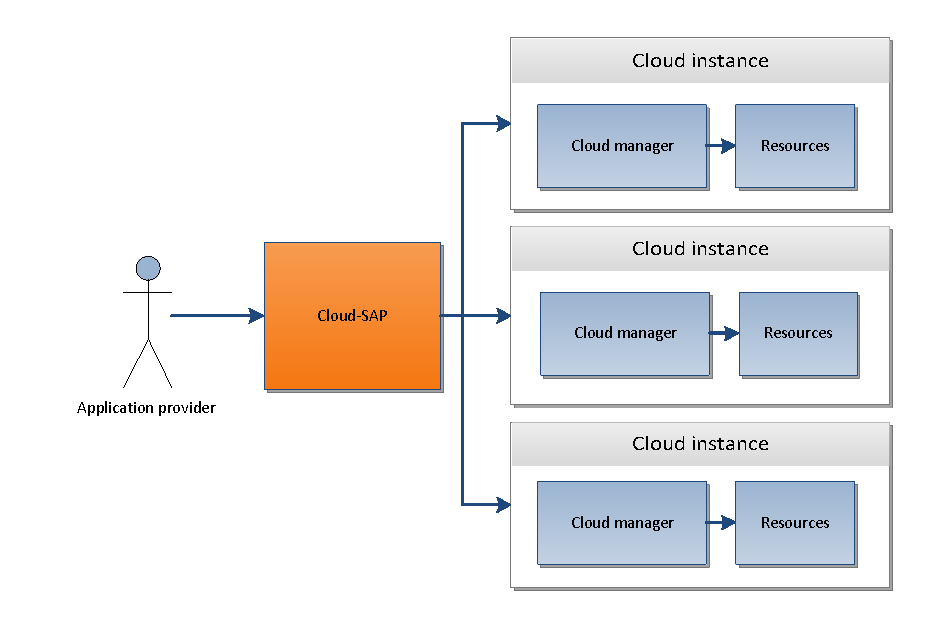
\includegraphics[width=0.9\textwidth]{chapter-design/architecture-context}
  \end{center}
  \caption{Cloud-SAP place in an exemplary application provisioning request}
  \label{img:architecture-context}
\end{figure}

Service consumers can be both end-users or other system interfaces, Cloud-SAP is suitable for both cases. Cloud-SAP is entirely cloud provider and resources agnostic as long as they externalise management interfaces.

Successive sections define core layers of a Cloud-SAP and give insights into possible implementation decisions, while the next chapter presents proof-of-concept implementation.

\section{Overview}
Przedstawienie domeny - zasobow w naszym systemie, odniesienie tego do blueprint => wynikiem jest pomysl na system / diagram

ogolny opis systemu - jak sie odnosimy do CHOP, mamy 1 kontroler orkiestrujacy, kompletny system autonomiczny

\begin{figure}[!ht]
  \begin{center}
    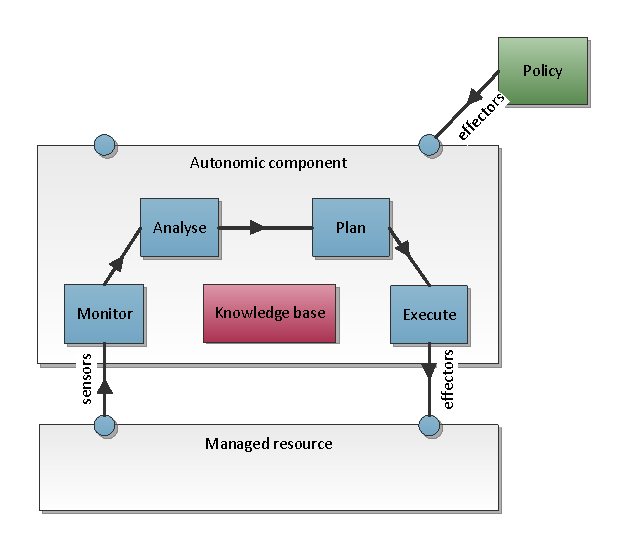
\includegraphics{chapter-design/autonomic-component}
  \end{center}
  \caption{autonomic component}
  \label{img:autonomic-component}
\end{figure}

\begin{figure}[!ht]
  \begin{center}
    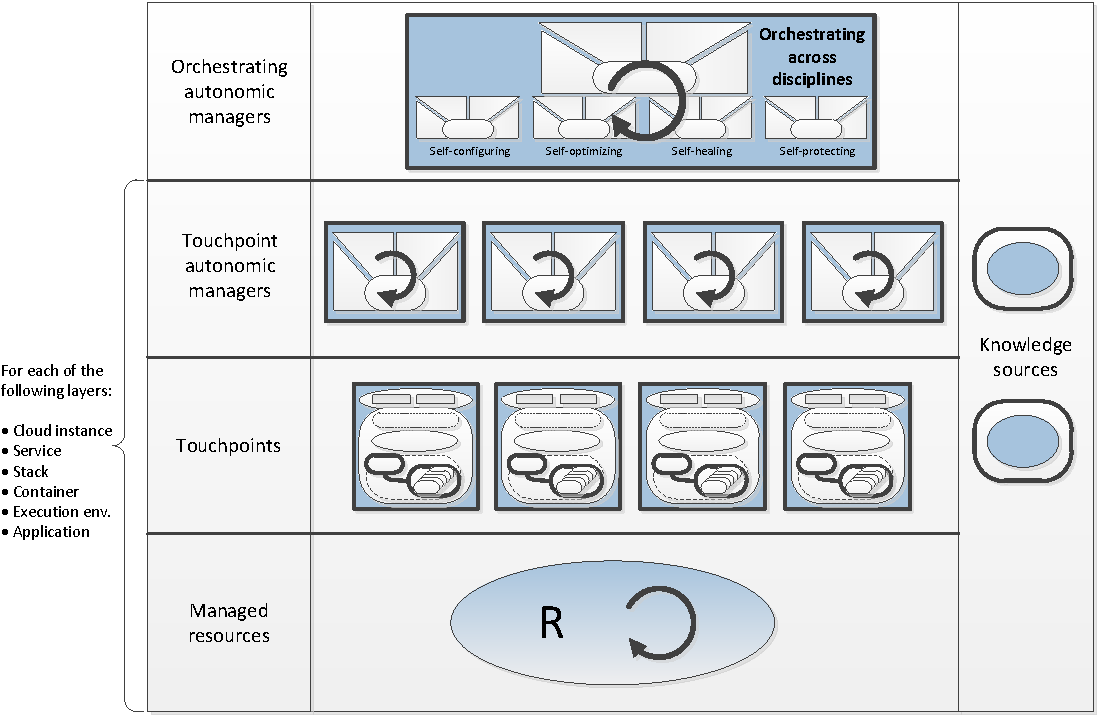
\includegraphics[width=\textwidth]{chapter-design/csap-layers}
  \end{center}
  \caption{autonomic component}
  \label{img:csap-layers}
\end{figure}

% darek
%\section{Application platform manager}
%w kazdej sekcji opis MAPEK - co monitoruje, w jaki sposob analizuje i planuje, wykonuje

% darek
\section{Autonomic container manager}
It is expected that autonomic container manager supervises lifecycle of a container, modifying its properties accordingly to a current demand.

\subsection{Managed resource}
Container is an entity that provides an execution environment for an application platform. Whilst Cloud-SAP is a hypervisor agnostic, it is recommended to use operating system level virtualization technique instead of a full virtualization as a underlying mechanism for a container provisioning. Lightweight containers are more suitable for our needs especially because we rely entirely on Linux based operating system. Hence, it not necessary to use hardware-based hypervisor that supports other operating systems. Moreover, lightweight containers have been proved more effective in some scenarios: \cite{RaHiSj13}.

Container uses variety of underlying resources such as storage or network connection. However, for a simplicity, Cloud-SAP doesn't require autonomic container manager to manage them.

\subsubsection{Touchpoint}
Container's touchpoint externalises hypervisor and operating system APIs. Similarly to all touchpoints, two main parts can be distinguished:
\begin{itemize}
 \item \emph{sensors} - set of properties that expose system metrics such as CPU, memory, disk usage, network bandwidth
 \item \emph{effectors} - a collection of 'set' operations that aims to change container state: increase or decrease CPU or memory, for example. In fact, these operations directly corresponds to hypervisor capabilities.
\end{itemize}

It is highly recommended for sensors and effectors to be linked, forming together manageability capabilities. In other words, property (i.e. CPU) can be read only when it is possible to set it as well. 

\subsection{Autonomic controller}
Generally speaking, autonomic container controller aims to automate container's management function and externalise its configuration through its interfaces. In order to do achieve that, it implements a control loop that fully covers container life cycle: gathering information about it, analysing it, planning and executing actions on top of that. These four functions along with knowledge necessary to perform them designate modular structure of a controller as shown in figure \ref{img:autonomic-component}.

\subsubsection{Monitoring}
As it was already mentioned, monitoring module aims to gather data from container's sensors. While design of Cloud-SAP doesn't have any specific requirements regarding underlying monitoring mechanism, there are a few aspects that should be taken into consideration:
\begin{asparaenum}
  \item[\textbf{Data filters}]

  \item[\textbf{Persistence}]

  \item[\textbf{Standard compatibility}] Whilst there is no single, industry accepted standard of virtual machine monitoring, there were initiatives such as OCCI \cite{OCCI} that aims to close that gap. Having scaling across multiple cloud instances in mind, it is vital to provide compatibility at a container monitoring level. However, in some cases, standard-defined API may no be sufficient for a specific needs  
\end{asparaenum}


\subsubsection{Analysis}
\subsubsection{Planning}
\subsubsection{Execution}
\subsubsection{Knowledge}

% darek
\section{Autonomic stack manager}

% radek
\section{Autonomic cloud instance manager}

% radek
\section{Autonomic cloud federation manager}

\section{Summary}
podsumowanie, wyzwania stojace przed projektem, problemy ale takze obietnica dobrobytu i spokojnej starosci
